\documentclass[a4paper,english,12pt,bibliography=totoc]{scrreprt}

\usepackage[T1]{fontenc} %immer
\usepackage[utf8]{inputenc} %am
\usepackage{babel} %Anfang
\usepackage{wasysym}

\usepackage{enumitem} %Aufzählungen verändern
\usepackage[
backend=biber,
style=alphabetic,
sorting=ynt
]{biblatex}

\addbibresource{Reference.bib}
\bibliography{Reference}
%Gleichungen verwenden
\usepackage{newtxtext}
\usepackage{amsmath}
\usepackage{amssymb}
\usepackage{mathptmx}
%\usepackage{txfonts}

\usepackage{listings}% code blocks
\usepackage[most]{tcolorbox}

%Querverweise
\usepackage{varioref} %immer
\usepackage{hyperref} %in dieser
\usepackage{cleveref} %Reihenfolge

\usepackage{booktabs} %schönere Tabellen
\usepackage{siunitx} %SI-Einheiten
\usepackage{tabularx} %Tabellen mit flexiblen Spalten	

\usepackage{graphicx} %Grafiken verwenden

\usepackage{lipsum} %Blindtext
\usepackage{wrapfig} %wrapfig
\usepackage{subcaption}
\usepackage{afterpage}
\usepackage[headsepline]{scrlayer-scrpage} %Paket für Kopfzeilen
\usepackage{afterpage}
\usepackage{float}
\automark[subsection]{section}

\pagestyle{scrheadings}
\ihead{} % oben links
\chead{\leftmark} % oben Mitte
\ohead{} % oben rechts
\cfoot{\pagemark} % unten Mitte
\automark[section]{section} % Modified line

% Zu volle hboxen korrigieren
\tolerance 1414
\hbadness 1414
\emergencystretch 1.5em
\hfuzz 0.3pt
\widowpenalty=10000
\vfuzz \hfuzz
\raggedbottom

%Informationen über das Dokument
\date{\today}


\begin{document}


\begin{titlepage}
	\centering
	
\includegraphics[width=0.8\textwidth]{logo_uulm_sw}
	
	\vspace{1cm}
	\LARGE Laboratory Module for Master Programs
	\Huge \textbf{Biophysics Lab Course}
	
	\vspace{1cm}
	\Large Experiment: 

	\Huge \textbf{Single molecule FRET}
	
	\vspace{15mm}
	\Large Performed on 
	
	\vspace{5mm}
	\LARGE Group 8
	
	\vspace{1cm}
	\Large
	\begin{tabular}{rcl}
	\textbf{Haiyang Zhang} & and & \textbf{Nicolae Turcan}\\
	\href{mailto:student.1@uni-ulm.de}{haiyang.zhang@uni-ulm.de} & & \href{mailto:student.2@uni-ulm.de}{nicolae.turcan@uni-ulm.de}
	\end{tabular}
	
	\vspace{7mm}
	Supervisor: Susanna Dalla Longa
	
	\vfill
	\begin{tabular}{p{50mm}@{\hspace{5cm}}p{50mm}}
	\hrulefill & \hrulefill \\
	%\centering Haiyang Zhang  & \centering Nicolae Turcan
	\end{tabular}
	
	\vspace{5mm}
	\normalsize \raggedright
	We hereby confirm that we have elaborated the present work independently and have detailed knowledge of the entire contents.
\end{titlepage}



\tableofcontents

\chapter{Abstract}
\label{cha:abstract}

In this study, we utilized Förster resonance energy transfer (FRET) and Total Internal Reflection Fluorescence (TIRF) microscopy to investigate single DNA molecules. FRET enables nonradiative energy transfer between donor and acceptor fluorophores, revealing molecular distances. TIRF microscopy selectively excites fluorophores near a surface, enabling sensitive detection. Experimental procedures involved DNA sample preparation, chamber setup, and data acquisition. Analysis with MATLAB software provided insights into donor-acceptor dynamics.


\chapter{Introduction}
\label{cha:Introduction}

\section{Single molecule Fluorescence}
Single-molecule spectroscopy has been widely used in biological research. It could help us explore the properties of the single molecule, which might be hidden under the average ensemble properties. In this experiment, we observed the DNA molecule on a single molecule level with the help of Förster resonance energy transfer(FRET) and Total internal reflection fluorescence(TIRF).

\section{Förster resonance energy transfer(FRET)}

One important process that could occur in the excited state is FRET, the nonradiative energy transfer from an excited molecule(donor) to another fluorophore(acceptor) by dipole-dipole coupling. \\

The energy transfer process can be explained by Jablonski diagram(Figure 2.1). In this process, a donor accept a photon, excited from state $\mathrm{S_0}$ to $\mathrm{S_1}$ (Green arrow). The energy could transfer to acceptor fluorophore from donor via nonradiative process (Yellow arrow). Finally, the energy level of acceptor transfers from $\mathrm{S_1}$ to $\mathrm{S_0}$, with the emission of a photon (Red arrow).\\

\begin{figure}
    \centering
    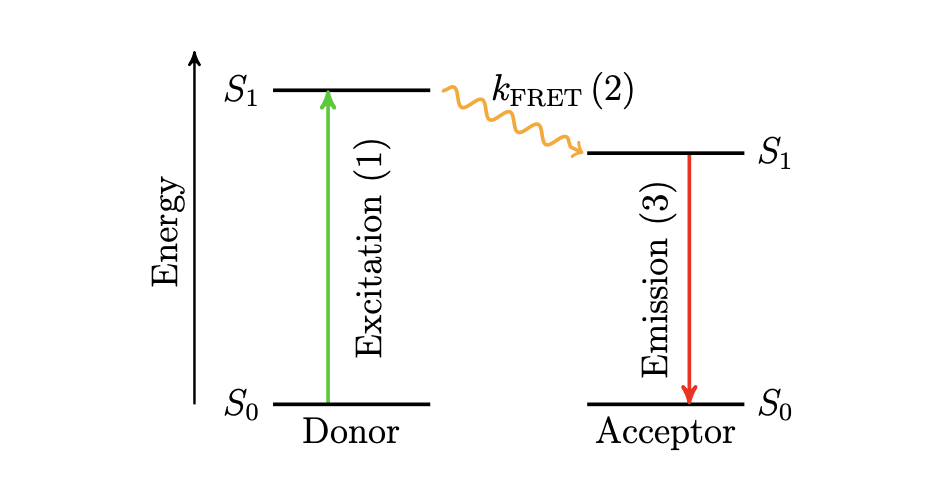
\includegraphics[width = 0.9\textwidth]{images/FRET Jablonski.png}
    \caption{The Jablonski diagram of FRET process}
\end{figure}

\begin{figure}
    \centering
    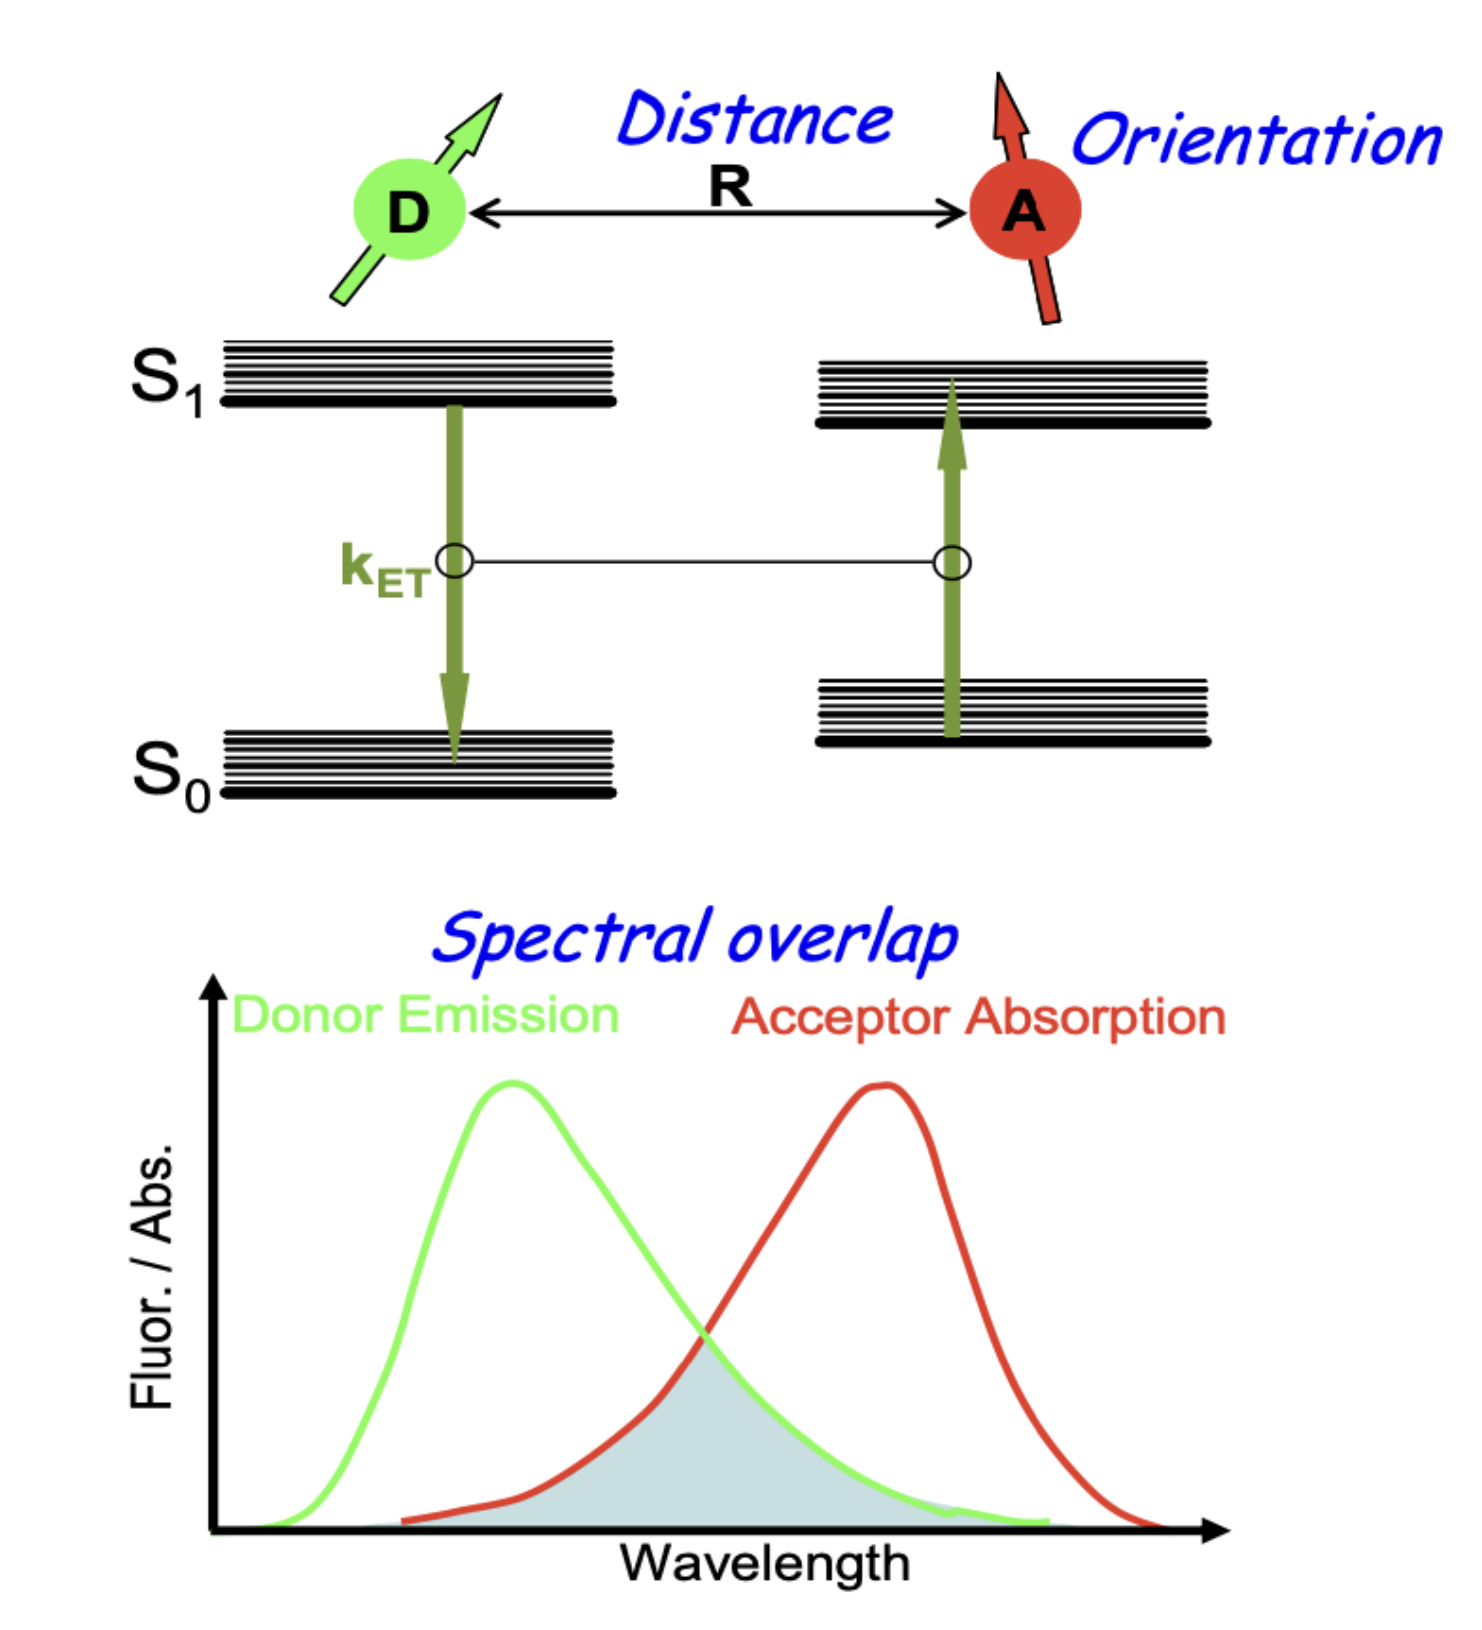
\includegraphics[width=0.9\textwidth]{images/FRET theory.png}
    \caption{Steric and energetic conditions for efficient Föster transfer\cite{Fluorescence_lifetime_lab_script}}
    \label{fig:enter-label}
\end{figure}
There are several requirements that need to be fulfilled for FRET. First, the donor and acceptor fluorophores have to be in close proximity, which in general, is less than 10 nm. Additionally, the donor and acceptor dipole orientations must be approximately parallel. Furthermore, the emission spectrum of the donor has to overlap with the absorption spectrum of the acceptor, as is shown in figure 2.2. And the distance dependence of the rate coefficient for energy transfer is found to be:
\[
k_{FRET}(R) = \frac{1}{\tau_D}(\frac{R_0}{R})^6
\]
and
\[
R_0 = (\frac{9ln(10)\kappa^2\phi_DJ}{128\pi^5N_An^4})^{1/6}
\]
\\
Here $k_{FRET}$ is the rate coefficient of FRET, and $R_0$ is called Förster radius, which characterizes the FRET pair. The $\phi_D$ is the fluorescence quantum yield of the donor, n is the refractive index, $\kappa^2$ is the orientation factor, and J is the overlap integral, which is:
\[
J = \int \epsilon_A(\lambda)f_D(\lambda){\lambda}^4\, d\lambda
\]
For practical calculations, we use the following formula:
\[
R_0 = 0.0211(J\kappa^2n^{-4}\phi_D)^{1/6}
\]


Here, the unit of the Föster radius is nm, while the unit of J is $(M \cdot cm)^{-1}$ and the wavelength in nm.\\

The energy transfer efficiency E is defined for the further calculation. When $R = R_0$, the efficiency should be 50\%. By definition, it is:
\[
E = \frac{k_{FRET}(R)}{k_{FRET}(R) + k_F + k_{nr}} = \frac{1}{1+(\frac{R}{R_0})^6}
\]
Because it is highly sensitive to the distance, FRET can be used to determine the distance around $R_0$ of the dye pair on the nanometer scale.\\

In this experiment, the distance R between two fluorophores(Cy3B and Alexa647) attached to the double-stranded DNA was determined by measuring the FRET efficiency of this sample, and the Förster radius $\mathrm{R_0} = 68$ \AA \ was determined previously.
\section{Total internal reflection fluorescence(TIRF)}
TIRF is a common method in single molecule FRET research. It is based on the optical phenomenon that an evanescent field will be generated while the refraction light changes to total reflection light between two different media with two distinct refractive indices.

\begin{figure}
    \centering
    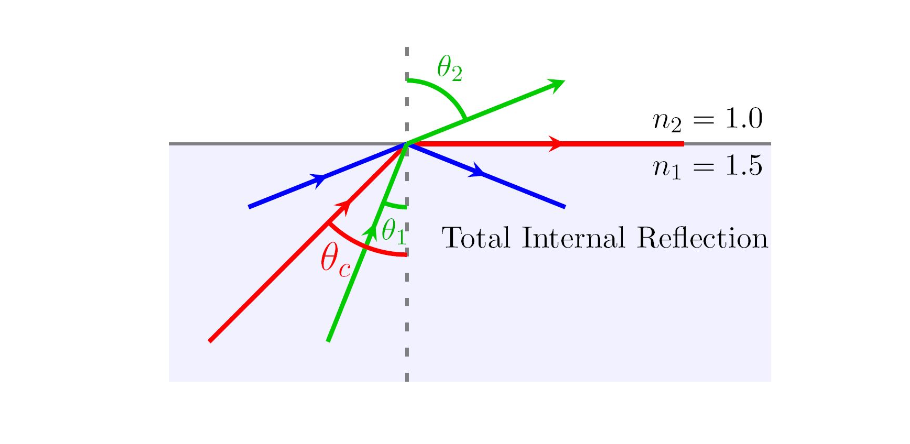
\includegraphics[width = 0.9\textwidth]{images/TIRF.png}
    \caption{The sketch of optical phenomenon of total internal reflection}
\end{figure}

As the sketch(Figure 2.3) shown, the green beam of light passes from a medium with higher refractive index $n_1$ to a boundary surface of a medium with lower refractive index $n_2$. The angle of refracted light is described by Snell's law
\[
n_1 sin\theta_1 = n_2 sin\theta_2
\]
And when the incident angle is larger than the critical angle $\theta_c$, the electromagnetic wave can no longer penetrate the medium with lower refractive index, and eventually become total reflected beam(the blue path).\\
\begin{wrapfigure}{r}{0.45\textwidth}
    \centering
    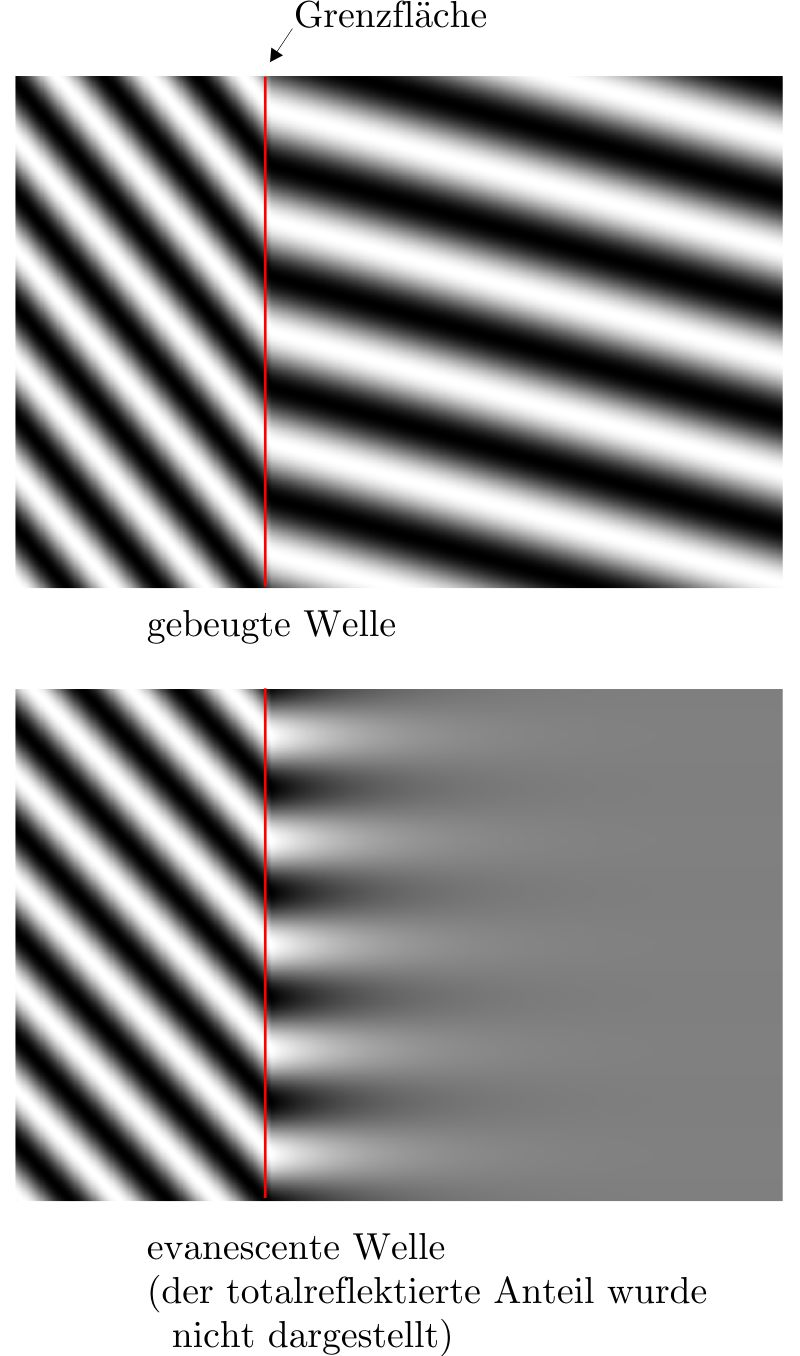
\includegraphics[width = 0.4\textwidth]{images/Evanescent_wave.jpg}
    \caption{The refraction wave (up) and the evanescent wave (down). \cite{article}}
\end{wrapfigure}
Except for the reflected waves, an evanescent wave is generated at the boundary surface(Figure 2.4). This evanescent wave reaches its maximum intensity at the surface and then exponentially decays with the depth of the medium. Therefore, this characteristic of evanescent wave allows us to only excite the fluorophores near the surface (within 100nm approximately), and it could also decrease the background signals of the bulk solution, which allows sensitive detection on single molecule scale.
\chapter{Material and Methods}
\label{cha:MaterialandMethods}
In the following sections the materials and methods will be discussed.
\section{Material}
\label{sec:material}
The following Table 3.1 the Materials used in the experiment are presented. 

\begin{table}[h]
\centering
\caption{Materials for Experiment}
\begin{tabular}{ll}
\toprule
\textbf{Material} & \textbf{Details} \\
\midrule
%Glass Slides & with Syringe ports attached for fluidics \\
%1mm $\diameter$ plastic tube & attached to inlet and outlet of chamber\\
1mL Syringe & Equipped with 20 Gauze needle \\
%Glass Covers & Wide \\
%Nescofilm & Thin layer for creating the flow cell\\
%Fluidics Chamber holder & for simple mounting on optical table \\
%532nm DPSS Laser & Diode-Pumped Solid State Laser (532 nm) \\
%Lens 1 & for collimating the laserbeam \\
%3 Kinematic Mirror Holders & Holders for precise beam positioning \\
%Lens 2 & for focusing the beam trough the prism\\
%TIR Prism & Prism for Total Internal Reflection Fluorescence microscopy \\
%Micrometer XYZ stage & allowing movement in XYZ-direction\\
%Water Immersion Objective & 60x magnification \\
%Lens 3 & for collimating the beam before the slit\\
%Single Slit & for cutting the image in half \\
%Lens 4 & for focusing the beam on the beam splitter\\
%Dichroic beam splitter & DC Chroma 645 DCXR\\
%Filter 1 & F1 Semrock FF01-582/75 \\
%Filter 2 & F2 Chroma HQ665/65 \\
%Lens 5 & for focusing the image on the sensor\\
%EMCCD camera & Electron Multiplying Charge-Coupled Device  \\
%Eppendorfs & 1.5mL capacity \\
Neutravidin & in solution 1 mM \\
dsDNA Mixture & Contains 50:50 DNA samples with 2 FRET distances (Cy3B-Alexa647) \\
HMNE Buffer & a mix of buffer solutions for DNA experiments\\
PBS & Phosphate Buffer Solution \\




\bottomrule
\end{tabular}
\end{table}


\section{Methods}
\label{sec:methods}

\subsection{Experimental Setup of Prism-Type TIRF Microscope}
The experimental setup of the prism-type TIRF microscope involves distinct pathways and components to facilitate the imaging process.
\subsubsection{Excitation Pathway}
The excitation pathway employs a Diode-Pumped Solid State (DPSS) Laser emitting monochromatic light at 532 nm. This laser is equipped with controllers for temperature and power adjustments. By collimating the laserbeam with a lens (L1), deflecting it with three mirrors, and focusing it with another lens (L2) onto the sample chamber through a prism (P), the excitation light is directed at the sample at an appropriate Total Internal Reflection Fluorescence (TIRF) angle.
\subsubsection{Sample-Holding Stage}
To host the biological sample, a glass slide sealed with Nescofilm to a cover slip is mounted onto a specialized holder in advance.
\subsubsection{Sample Chamber}
Chapter 4.2 elaborates on the meticulous procedure for preparing and immobilizing the sample within the chamber, which is affixed to a micrometer stage allowing movement in XYZ-direction.
\subsubsection{Emission Pathway}
Fluorescence emitted by the sample is captured through a water-immersion objective and directed to an Electron Multiplying Charge-Coupled Device (EMCCD) camera. A slit (S) strategically positioned within the image plane partitions the fluorescence to cover only half of the camera chip, enabling simultaneous imaging of donor and acceptor fluorescence.
\subsubsection{Dichroic Beam Splitter}
A dichroic beam splitter (DC) segregates the donor and acceptor fluorescence based on their distinct emission spectra. This mechanism facilitates effective separation, ensuring precise imaging.
\subsubsection{Filters}
To enhance specificity, suitable filters (F1: Semrock FF01-582/75, F2: Chroma HQ665/65) are employed post-dichroic to block unwanted wavelengths, optimizing signal-to-noise ratio.
\subsubsection{Camera Setup}
The final lens (L5) directs the segregated fluorescence beams to occupy one half of the camera chip, facilitating simultaneous observation of donor and acceptor fluorescence channels via dedicated software on the computer.

In the following Figure 3.1 we display a visual representation of the optical setup described above.

\begin{figure} [H]
    \centering
    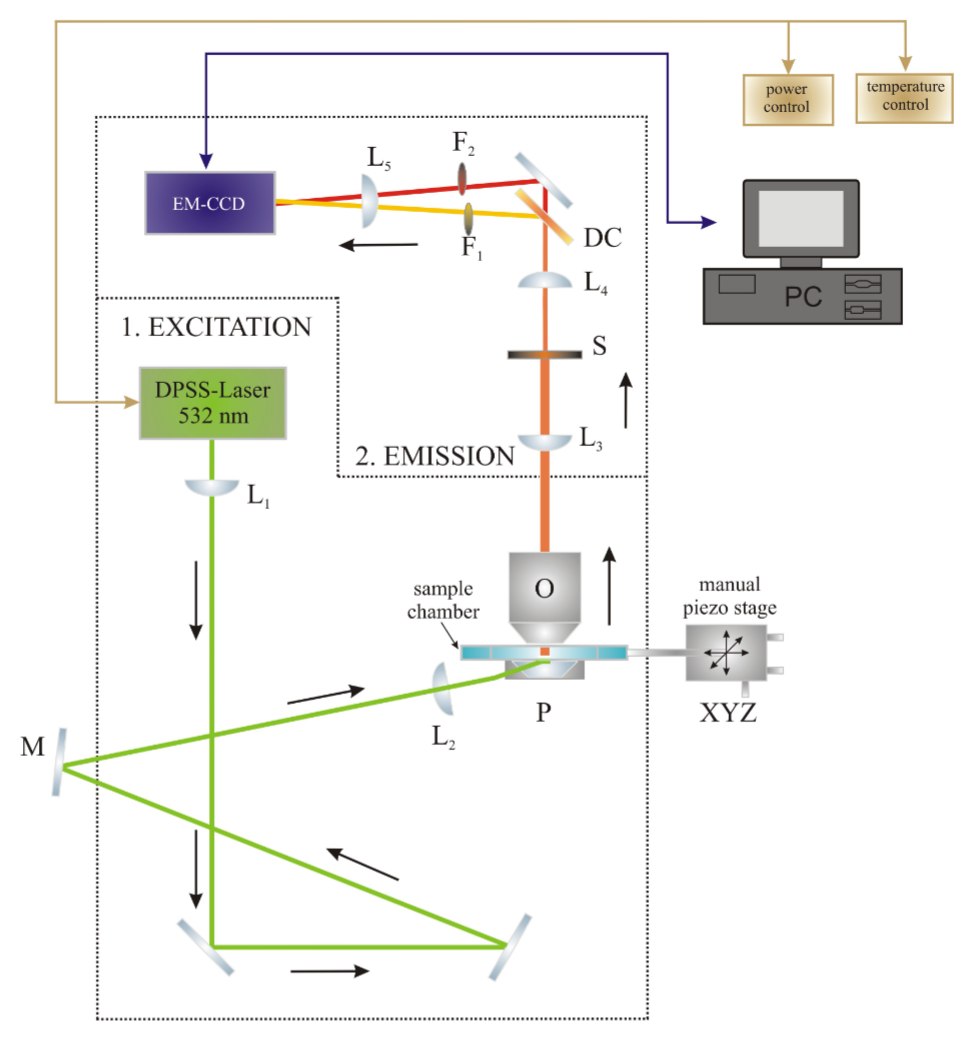
\includegraphics[width=0.8\linewidth]{opticalsetup.png}
    \caption{Optical Setup Representation}
    \label{fig:enter-label}
\end{figure}

\subsection{DNA Sample Immobilization}

The initial step involves immobilizing the DNA sample onto the quartz glass surface within the sample chamber. Prior to the practical session, the sample chambers are meticulously prepared. Each chamber comprises a quartz slide treated with biotinylated polyethylene glycol (PEG), a cover slip, and a layer of Nescofilm (approximately 120 $\mathrm{\mu}$m thick) sandwiched in between. This assembly forms a functional flow chamber.

\subsubsection{Neutravidin Incubation}

To facilitate binding of the biotinylated DNA to the surface, the chamber undergoes incubation with Neutravidin, a tetrameric protein featuring four binding sites known for its robust affinity for biotin.


\begin{figure} [H]
    \centering
    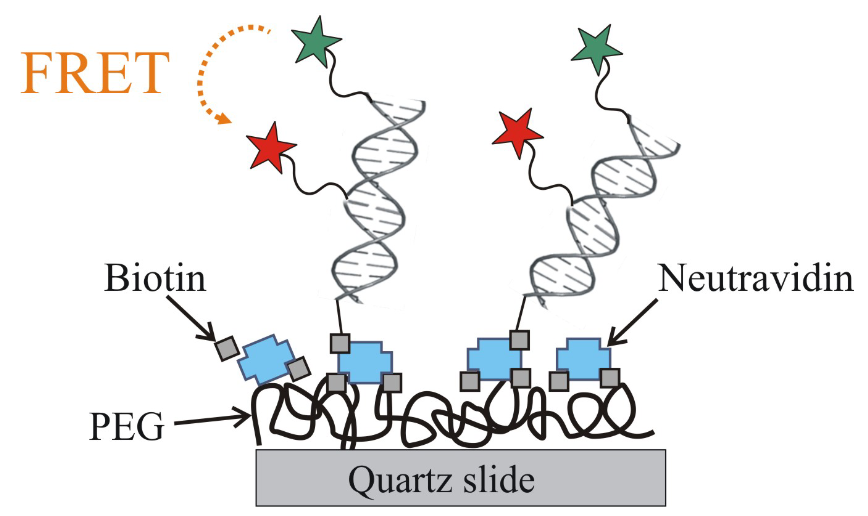
\includegraphics[width=0.8\linewidth]{images/quartslide.png}
    \caption{Quartz Slide surface}
    \label{fig:enter-label}
\end{figure}

\paragraph{Procedure}

\begin{enumerate}
    \item Prepare 800 $\mu$L of PBS buffer, 600 $\mu$L of HMNE buffer, and 100 $\mu$L of Neutravidin.
    \item Attach a 1 mL syringe with needle to the outlet tubing of the chamber, and immerse the inlet tubing into the PBS Eppendorf.
    \item Gently draw 0.3 mL of PBS through the chamber using the syringe, ensuring the absence of air bubbles.
    \item Shift the inlet tubing from the PBS Eppendorf, gently press the syringe to form a drop at the inlet tubing, then insert the inlet tubing into the Neutravidin Eppendorf to prevent air ingress.
    \item Disconnect the syringe with the needle from the outlet tubing and gradually flush the chamber with Neutravidin, administering it drop by drop.
    \item Invert the chamber and let it incubate at room temperature for 15 minutes.
\end{enumerate}

\subsubsection{Preparation of DNA Dilutions}

Post-incubation, prepare 100 $\mathrm{\mu}$L solutions of the provided 1 $\mu$L DNA mixture in HMNE buffer, with dilutions ranging from 1:100 to 1:$10^5$.

\subsubsection{Final Flush}

Conclude the preparation process by flushing the chamber sequentially with PBS and HMNE.



\chapter{Experiment and Analysis}
\label{cha:experimenandanalysis}  

\section{Experiment}
\label{sec:experiment} 

%\subsection{Preparation of DNA samples}
In this experiment, a DNA mixture labeled with Alexa647 and Cy3B was used. The mixture contained two types of DNA samples with different donor-acceptor distances, with a theoretical ratio of 50:50. Four groups of DNA dilutions(from 1:100 too 1:$10^5$) were made(see 3.2.2) for the further experiment.\\

A chamber was pre-prepared and treated to immobilize the DNA (see 3.2.2) for this experiment. After the incubation, it was attached to the 3-axis stage. A prism coated with immersion oil was mounted on the prepared chamber construction (see figure 4.1), and a water drop was put between the chamber and objective. Till now, all necessary devices are settled.\\

The next thing was adjusting the optical path. The first thing was correcting the z-position of the chamber. The correction z-position was determined by using an auxiliary laser beam path(figure 4.2). Two flipping mounts were turned into the beam as is shown in the figure. Then we switched on the laser and put a piece of paper behind the 50:50 beam splitter to visualize the laser beam coming back from the objective. By moving the chamber gently, we observed that the laser beam was focused three times, and the third focus point, which represented the surface of the quartz glass where the DNA molecules were immobilized, was the point we needed. \\

After that, the camera program (coded by Andor Luca) was turned on and only background noise could be observed. The location of the laser beam was adjusted using the tunnel outside the box until comparatively light and dark background was displayed on the monitor. Then the laser was turned off and DNA dilution was loaded into the chamber. After 2~5 minutes, the laser was turned on again for us to determine the proper dilution of DNA by observing the density of the fluorophore shown on the monitor.\\

After we found the suitable dilution, we started to acquire the movies. The x positioner was used to find a new spot, and the z positioner was used to slightly correct the focus. A .sif document would be generated after the filming. And this process was repeated many times until we acquired enough movies for analysis.
%800$\mu$L PBS buffer, 1000 $\mu$L HMNE(instead of 600 $\mu$L) and 100 $\mu$L Neutravidin were maintained for the experiment. Then, 1 $\mu$L of DNA mixture was taken out, and diluted to 1:100 DNA solution( 100 $\mu$L) by addition of HMNE buffer. Then, 10 $\mu$L of this DNA solution was taken out, and diluted to 1:1000 DNA solution (100 $\mu$L) by the addition of HMNE buffer again. This process was repeated to produce four DNA samples($1:100, 1:10^3, 1:10^4, 1:10^5$).\\
\begin{comment}
    

\subsection{Setting up the sample chamber}
A sample chamber was pre-prepared(See material and methods). In the experiment, a 1 mL syringe was used to put the solutions into the chamber. The syringe was attached to the outlet tubing of the chamber. The first step is to put the inlet tubing into the 1 mL PBS Eppi. Then, 0.3 mL of PBS was pulled in the chamber slowly and evenly to avoid the air bubbles in the chamber. After that, the inlet tubing was taken out from the PBS Eppi, and a drop was created by pushing the syringe in order to prevent the air enter the chamber.

The next step is to flush the chamber by Neutravidin. After the processes above, the inlet tubing was put into the Neutravidin Epi. And by pulling the syringe very slowly, the chamber was flushed by the Neutravidin drop by drop. \\

Then the chamber was put upside down at room temperature about 15 minitues for incubation. After the incubation, the chamber was flushed again with PBS and HMNE drop by drop. After that, the chamber was fixed on the 3-axis stage. Then the chamber was carefully moved very close to the objective with the z-positioner of the stage. A prism coated with immersion oil is mounted on the prepared chamber construction, and a water drop was put between the chamber and the objective(figure 4.1). Finally, when the TIRF adjustments were done, 200 $\mu$L HMNE buffer and DNA dilution was pulled into the chamber. After 2-5 minutes, the measurement could start. 
\end{comment}
\begin{figure}
    \centering
    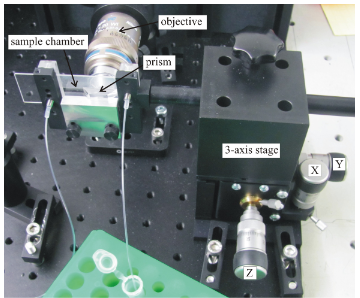
\includegraphics[width = 0.95\textwidth]{images/Bulit in chamber with prism on micrometer stage in front of the objective.png}
    \caption{The position of chamber and prism on micrometer stage in front of the objective}
\end{figure}
\begin{comment}
    

\subsection{Measurement and collecting the data}

At least ten minutes before the measurement start, the laser power and the temperature controller was turned on. The first thing we did was correcting the z-position of the chamber. The correction z-position was determined by using an auxiliary laser beam path(figure 4.2). Two flipping mounts were turned into the beam as is shown in the figure. Then we switched on the laser and put a piece of paper behind the 50:50 beam splitter to visualise the laser beam coming back from the objective. By moving the chamber gently, we observed that the laser beam was focused three times, and the third focus point was the point we needed. It represented the surface of the quartz glass where the DNA molecules were immobilised.\\

After that, the camera program( coded by Andor Luca) was turned on, by clicking the live image, the background image of laser beam could be observed. Then with the help of advisor, the location of the laser beam was adjusted using the tunnel outside the box. Comparatively light and dark background was displayed on the monitor. The laser was switched off for loading the DNA sample. After that, the laser was turned on again, in order to decide if it is the suitable DNA dilution.\\

When the suitable DNA dilution was loaded, we tried to acquire the movies. After the chamber was moved to a new spot, the molecules had shifted out of focus, losing their sharp and round appearance and becoming distorted. This was rectified by adjusting the z-positioner either forward or backward. However, it was crucial that this adjustment didn't take too much time, as once the spot in the chamber was illuminated, the donor fluorophores were promptly excited and began transferring their energy or even photobleaching. Therefore, the focus had to be quickly established, followed by an immediate recording of a movie by activating the photocamera in the Andor software. Throughout the 40-second acquisition period, it was imperative that nothing was disturbed on the setup or table to prevent defocusing or drifting of the chamber relative to the camera.\\

The movies were saved as .sif file, and analysed by the MATLAB codes(see analysis).
\end{comment}

\begin{figure}
    \centering
    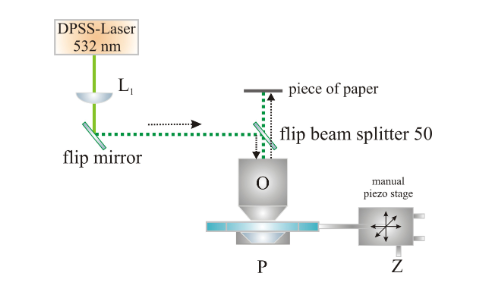
\includegraphics[width = 0.9\textwidth]{images/auxiliary laser beam.png}
    \caption{Schematic overview of the auxiliary laser beam path(dotted) which is needed to find the correct z-position of the chamber}
\end{figure}
\section{Analysis}
\label{sec:analysis} 
The data analysis is based on the MATLAB software written in the group of Prof.Michaelis, which could find the FRET pairs automatically, calculate and subtract the local background, and compute fluorescent trajectories\cite{smFRET_lab_script}. \\

As is shwon in figure 4.3, the time traces of donor and acceptor were presented and divided into 3 phases. In phase I, both donor and acceptor were active and fluorescent. The green line (donor) is below the red line (acceptor) because FRET was taking place. Then in phase II, the acceptor intensity decreased abruptly due to bleach. Therefore, the energy transferred to the now bleached acceptor in the phase I was not transferred in phase II, so the photon emitted by donor increased rapidly, as the green line showed. And eventually all donor and acceptor were bleached, which was shown in phase III.\\

\begin{figure}
    \centering
    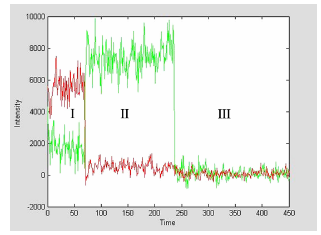
\includegraphics[width = 0.75\textwidth]{images/3 phases.png}
    \caption{FRET time trace of a donor (green) and acceptor molecule (red)}
\end{figure}

\begin{figure}
    \centering
    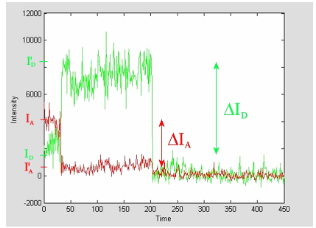
\includegraphics[width = 0.75\textwidth]{images/parameters.png}
    \caption{Characteristic FRET time trace of a donor (green) and acceptor molecule (red) showing the parameters $\Delta I_A$ and $\Delta I_D$ }
\end{figure}

The following formulas are used in the software to calculate the FRET efficiency:
\[
E_{FRET} = \frac{I_A - \beta \cdot I_D}{I_A + \gamma \cdot I_D}
\]
Where
\[
\gamma = \frac{\Delta I_A}{\Delta I_D} = \frac{I_A - I_A'}{I_D' - I_D}
\]
and
\[
\beta = \frac{I_A'}{I_D'}
\]

Here $I_A$ and $I_D$ are background correctiing intensities from donor and acceptor channels, and respectively, $I_A (I_D)$  and $I_A' (I_D')$ are intensities before (after) acceptor photon bleaching process. And the $\beta$ and $\gamma$ are experimental correction factors, where $\beta$ accounts for the leakage of the donor emission into the acceptor channel, and $\gamma$ includes the fluorescence quantum yields of the fluorophores and the detection efficiencies of the two channels.\\

Theoretically, our analysis should be based on the traces which could show these three phases clearly. Practically, however, we couldn't observe such ideal curve. Instead, we saved the curves with relatively clear separation between I and II areas. Finally, all FRET.only.txt files which contain the framewies FRET values of the selected molecules are combined together in one *.dat file which contains the efficiencies analyzed from the traces, and put into the Origin to get the histogram and double Gaussian fit. 


\chapter{Results and Discussion}
\label{cha:ResultsandDiscussion}

\section{Results}
\label{sec:Results} 
In our case , even after hours or recording and tweaking all the possible variables we had available to us, we couldn´t produce any results that enabled us to distinguish between the two DNA species. The details of the possible reason why this was the case for us will be cleared in the following section named discussion.
\newline
However, we were gently provided by our lab tutor with the results of a past experiment, in particular this experiment was performed over the course of multiple days by a group of Ph.D. students, therefore it can be considered as the best possible achievable result for this particular setup.\newline

by using the formula below and a known Förster radius of 68 Å we can compute the expected distances, which are given in table 5.1.

$$r = (1/E -1)^{1/6} R_o$$

In the table 5.1 the notation 1 and 2 refer to the radius of different FRET samples, while the f and m denote if they are from framewise (f) data or moleculewise (m) data.\\
\begin{table}[htbp]
\centering
\begin{tabular}{|c|c|}
\hline
Parameter & Value (nm) \\
\hline
$r_{1f}$ & $5.66$ \\
$r_{2f}$ & $6.92$ \\
$r_{1m}$ & $5.74$ \\
$r_{2m}$ & $6.90$ \\
\hline
\end{tabular}
\caption{Values of $r_{1f}$, $r_{2f}$, $r_{1m}$, and $r_{2m}$.}
\label{tab:values}
\end{table}

\begin{comment}
\[
r_{1f} = (\frac{1}{0.7508} - 1)^{1/6} \times R_0 = 5.66 nm
\]
\[
r_{2f} = (\frac{1}{0.4731} - 1)^{1/6} \times R_0 = 6.92 nm
\]
\[
r_{1m} = (\frac{1}{0.7508} - 1)^{1/6} \times R_0 = 5.74 nm
\]
\[
r_{2m} = (\frac{1}{0.7508} - 1)^{1/6} \times R_0 = 6.90 nm
\]
\end{comment}


The distance of a DNA basepair is around 3.4 \AA \cite{alberts2014}, and we can use this measure to compute the donor-acceptor distance in the number of basepairs for these two samples.
The computed values are provided in tables (a) and (b), and while the division operation gives a rational number (a), we should consider the closest integer to interpret the basepair distance (b).
\begin{comment}
    
The reason why we get non-integer values when using basepairs as a unit of measure could result from the fact that the basepair size used is just the mean value computed over an extremely long filament composed of thousands of individual basepairs with equal distribution. This allowed to make a measurement that wasn´t influenced so much by other factors( torsion, local interactions, h-bond length based on the pH of the environment, ecc...).
This was not the case for our short DNA sequences with large dye molecules attached, so a larger deviation from this mean is to be expected.
\end{comment}
\begin{table}[H]
\centering
\begin{subtable}[t]{0.4\linewidth}
\centering
\begin{tabular}{ll}
\toprule
\textbf{groups} & \textbf{distances} \\
\midrule
$d_{1f}$ & 16.65\\
$d_{2f}$ & 20.35\\
$d_{1m}$ & 16.88\\
$d_{2m}$ & 20.29\\
\bottomrule
\end{tabular}
\caption{The donor-acceptor distance divided by basepair distance}
\end{subtable}
\hspace{2cm} % Adjust the horizontal space between tables as needed
\begin{subtable}[t]{0.4\linewidth}
\centering
\begin{tabular}{ll}
\toprule
\textbf{groups} & \textbf{base pairs} \\
\midrule
$n_{1f}$ & 17\\
$n_{2f}$ & 20\\
$n_{1m}$ & 17\\
$n_{2m}$ & 20\\
\bottomrule
\end{tabular}
\caption{The donor-acceptor distances on the number of basepairs}
\end{subtable}
\end{table}

\begin{comment}
\begin{table}[h]
\centering
\begin{tabular}{ll}
\toprule
\textbf{groups} & \textbf{distances} \\
\midrule
$d_{1f}$ & 16.65\\
$d_{2f}$ & 20.35\\
$d_{1m}$ & 16.88\\
$d_{2m}$ & 20.29\\
\bottomrule
\end{tabular}
\caption{The donor-acceptor distance divided by basepair distance}
\end{table}

\begin{table}[h]
\centering

\begin{tabular}{ll}
\toprule
\textbf{groups} & \textbf{base pairs} \\
\midrule
$n_{1f}$ & 17\\
$n_{2f}$ & 20\\
$n_{1m}$ & 17\\
$n_{2m}$ & 20\\
\bottomrule
\end{tabular}
\caption{The donor-acceptor distances on the number of basepairs}
\end{table}
\end{comment}

\begin{comment}
    

\[
n_{1f} = 16.65
\]
\[
n_{2f} = 20.35
\]
\[
n_{1m} \approx 17
\]
\[
n_{2m} \approx 20
\]
\end{comment}


\begin{comment}
    

\begin{figure}[H]
    \begin{subfigure}{0.45\textwidth}
        \centering
        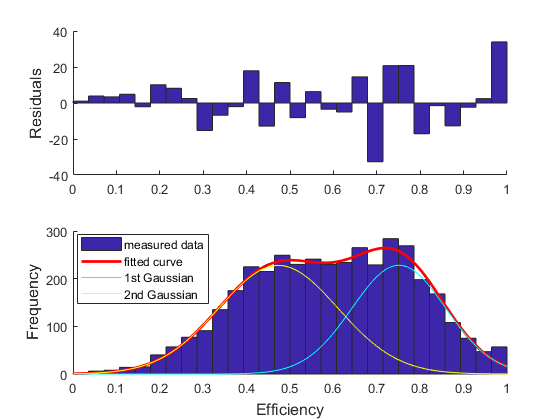
\includegraphics[width=\textwidth]{framewise_plot.png}
        \caption{the histogram and the double Gaussian fit for the framewise data}
    \end{subfigure}
    \begin{subfigure}{0.45\textwidth}
        \centering
        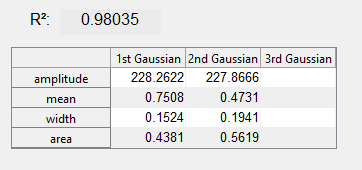
\includegraphics[width=\textwidth]{framewise_results.PNG}
        \caption{the fitting results of the double Gaussian fit of framwise data}
    \end{subfigure}
    \caption{The results of framewise data}
\end{figure}
\end{comment}

The provided results consist of the histogram and the double Gaussian fitted curves of the framewise and moleculewise data, which are shown in Figures 5.1 and 5.2. Here the framewise data means that many FRET efficiencies are collected and calculated from each frame, while the molecule-wise data is collected by just using the average intensity for each FRET pair and calculated once. In general, the framewise data is considered to be better because it is based on a large amount of points and more trustworthy. From the fitting results we could derive the distance between the acceptor and donor of these two different FRET samples.


\begin{figure}[H]
  \begin{subfigure}{0.45\textwidth}
    \centering
    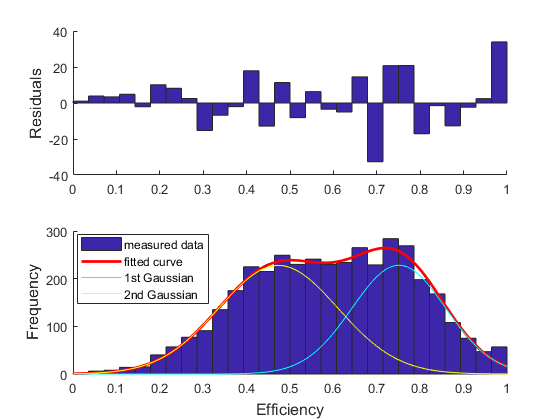
\includegraphics[width=\textwidth]{framewise_plot.png}
    \caption{The histogram and the double Gaussian fit for the framewise data}
  \end{subfigure}
  \begin{subfigure}{0.45\textwidth}
    \centering

    \begin{tabular}{lccc}
      $R^2 = 0.98035$ &  & \multicolumn{2}{c}{Gaussian} \\ \cline{3-4}
      & & 1st & 2nd \\ 
      \hline
      amplitude &  & 228.2622 & 227.8666 \\
      mean &  & 0.7508  & 0.4731 \\
      width  &  & 0.1524  & 0.1941 \\
      area &  & 0.4381  & 0.5619 
    \end{tabular}

    \caption{The fitting results of the double Gaussian fit of framewise data}
  \end{subfigure}
  \caption{The results of framewise data}
\end{figure}

\begin{comment}
    

\begin{figure}[H]
    \begin{subfigure}{0.45\textwidth}
        \centering
        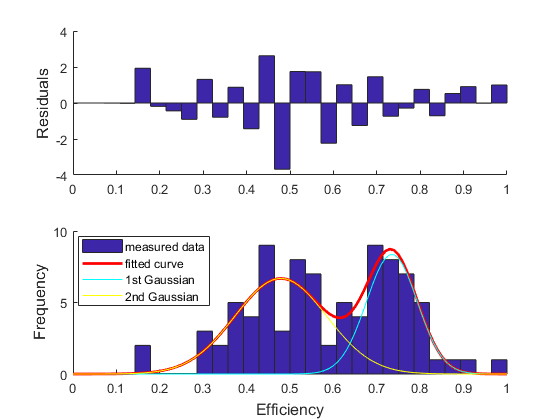
\includegraphics[width=\textwidth]{moleculewise_plot.png}
        \caption{the histogram and the double Gaussian fit for the single molecule data}
    \end{subfigure}
    \begin{subfigure}{0.45\textwidth}
        \centering
        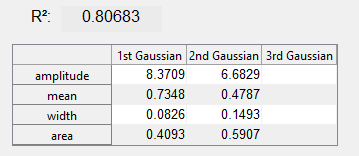
\includegraphics[width=\textwidth]{moleculewise_results.png}
        \caption{the fitting results of the double Gaussian fit of single molecule data}
    \end{subfigure}
    \caption{The results of single molecule data}
\end{figure}
\end{comment}

Condsidering these, we could divide our FRET samples into group 1 (with approximately 17 base pairs) and group 2 (with approximately 20 base pairs). And it is also possible to tell the real ratio of  molecules between the two samples. The area of the Gaussian curve represents the amount the number of one type of FRET among all the FRET samples. We could notice that the ratio between two areas, meaning the two different samples is not exactly 50:50. The ratio is approximately 44:56 for the framewise data and 41:59 for the moleculewise data.
This is to be expected since there could be some bias in the experimental setup, and the sample size is not big enough. If we were to continue recording events, we would most likely reach a 50:50 or otherwise increase our confidence in the presence of a bias in the system. 

\begin{figure}[H]
  \begin{subfigure}{0.45\textwidth}
    \centering
    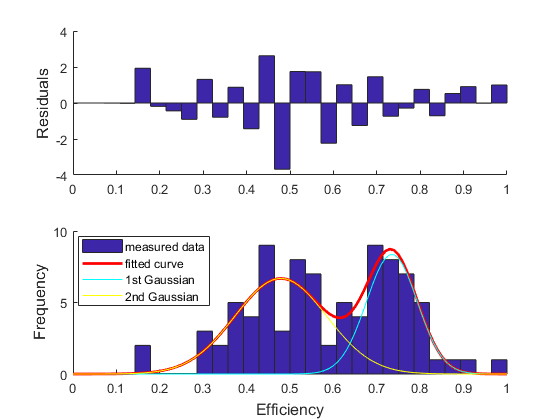
\includegraphics[width=\textwidth]{moleculewise_plot.png}
    \caption{The histogram and the double Gaussian fit for the framewise data}
  \end{subfigure}
  \begin{subfigure}{0.45\textwidth}
    \centering

    \begin{tabular}{lccc}
      $R^2 = 0.80683$ &  & \multicolumn{2}{c}{Gaussian} \\ \cline{3-4}
      & & 1st & 2nd \\ 
      \hline
      amplitude &  & 8.3709 & 6.6829 \\
      mean &  & 0.7348  & 0.4787 \\
      width  &  & 0.0826  & 0.1493 \\
      area &  & 0.4093  & 0.5907 
    \end{tabular}

    \caption{The fitting results of the double Gaussian fit of framewise data}
  \end{subfigure}
  \caption{The results of framewise data}
\end{figure}


\section{Discussion}
\label{sec:Discussion} 

Our experiment encountered several challenges, the most taxing challenge was the extremely fast photobleaching of our molecules, which in turn resulted in insufficient or partial recordings of the FRET events.
If we turned the laser intensity to the level written in the lab script, the fluorophores bleached extremely fast, and lowering the laser intensity would make the fluorophores invisible. It became almost impossible to get any figures that display the I, II, and III areas of the time trace clearly from the analyzed results. As a matter of fact, over multiple hours of conducting the experiment we managed to record only 2 or 3 time traces containing all three sections required for the calculations.
\\
Aligning the lenses accurately to focus the laser onto the sample proved to be a challenging task, it required multiple adjustments throughout the experiment. Precise alignment was crucial for obtaining any results at all, since no image will form on the plane of the camera otherwise.
\\Furthermore, identifying suitable fields of view where FRET events were occurring prominently was essential for capturing meaningful data and this is where the main challenges arose, because this task required careful observation when selecting a region with not too dense or sparse molecule distribution, all of this while needing to bring in focus the molecules as best as we could to improve the ability of the software to create pairings between the two recorded wavelengths. 
\\
The time-sensitive nature of the experiment exacerbated the challenges. The rapid photobleaching of dyes upon exposure to laser light necessitated swift operation to focus on the sample plane and capture FRET events before significant bleaching occurred or all the FRET pairs reached their third phase of the time trace.This  limited the duration of observation and added pressure to the experimental procedure.
\\
Moreover, typical sources of errors, such as mishandling the injection syringe setup for the sample chamber, could have influenced our results. Air bubbles in the sample chamber, resulting from improper handling, can disrupt the path of the laser light and introduce inconsistencies in recorded FRET event time traces. Manual selection of suitable time samples and identification of phase transitions in the time traces also introduced potential sources of error. This process requires expertise and experience, which we did not possess being the first time doing such an experiment.
\\
In summary, the challenges encountered during the experiment, including operational difficulties and potential sources of errors, underscore the complexity of single molecule studies. Addressing these challenges is crucial for improving the reliability of the technique and future research efforts should focus on refining the variable choice in the experimental protocols, such as dye choice, light intensity, presence of quenchers or even long-term stability of solutions and reagents.



    
\begin{comment}
    
\chapter{Conclusion}
\label{cha:Conclusion}
In this study, we acquired the distances between two dyes attached to DNA using  single molecule FRET from a mixture of two FRET samples.
\end{comment}

\printbibliography
\end{document}